\chapter{Blockchain Technologies}
\label{chap:blockchain}

\minitoc \mtcskip \noindent

This chapter introduces the most important concepts of blockchain which are essential for its applications. It interleaves the features of blockchain with its applicability to supply chain, by highlighting both the disadvantages and disadvantages, of blockchain in general and in particular to SCM, as well as any existing models for the integration of blockchain with SCM.

\section{Introduction}
“The Byzantine Generals' Problem” is a classical problem faced by distributed systems, which, in simple terms, states that consistency in a distributed system can never be fully guaranteed~\cite{byzantine-generals-problem}. This is derived from a lack of general consensus as to what the state of the system is at any given time.

Nakamoto's implementation of a blockchain seems to be, at present, the most practical way to approach this problem (though with its limitations), even earning the term "Practical Byzantine Fault Tolerance (PBFT) Algorithm", because of how it handles the consensus issue. The fact that many kinds of applications rely on distributed architectures, which might face these problems, turns blockchain all the more appealing. 
   
Some improvements have been built upon the traditional blockchain, such as smart contracts, which further enhance its use and allow for a wider variety of applications. Some areas where blockchain is starting to see some use include insurance, finance, Internet-of-Things, health care, identity management, to name a few.

In each of these areas, there are many ways in which blockchain can be used, be it to store information, process information, process payments or provide services. The versatility is what makes it so popular and what allows for the possibility of many other applications to be proposed.

\section{Core Concepts and Features}

%\paragraph{Original blockchain}    
The original blockchain, Bitcoin, was developed with the purpose of creating a distributed online payment system without the need for a financial institution or any other centralized trusted third party to verify the transactions. It even has its own currency, made up from digital tokens that represent real money, a concept which is now commonly known as a cryptocurrency.

Eventually, this concept evolved into something more, and new uses, other than online transactions, emerged from the blockchain technology. As described by Marc Pilkington~\cite{Pilkington2015}, \textit{"the essence of the blockchain is informational before being economic or monetary, conducive to many emerging and increasingly popular token-free blockchains"}.

Therefore, the algorithms used by Bitcoin are not a defining feature of the blockchain technology, but merely one of the many possible applications.
    
    The blockchain itself consists of a peer-to-peer network which continually stores and updates a chronological chain of blocks, where each block stores whatever information is relevant to the system in question, as well as the hash of the previous block. In the original blockchain, each block stored information about transactions between people, where there was a set of rules to check whether the transactions were valid or not. We'll get to how a blockchain can be built in a moment.
    
    One important and defining property of the blockchain is that the hash of the previous block also serves as an address. Therefore, each block has a pointer to the previous block, which is known as an hash pointer. This concept is illustrated in Figure~\ref{fig:blockchain_workflow}.
    
\begin{figure}[h]
\centering
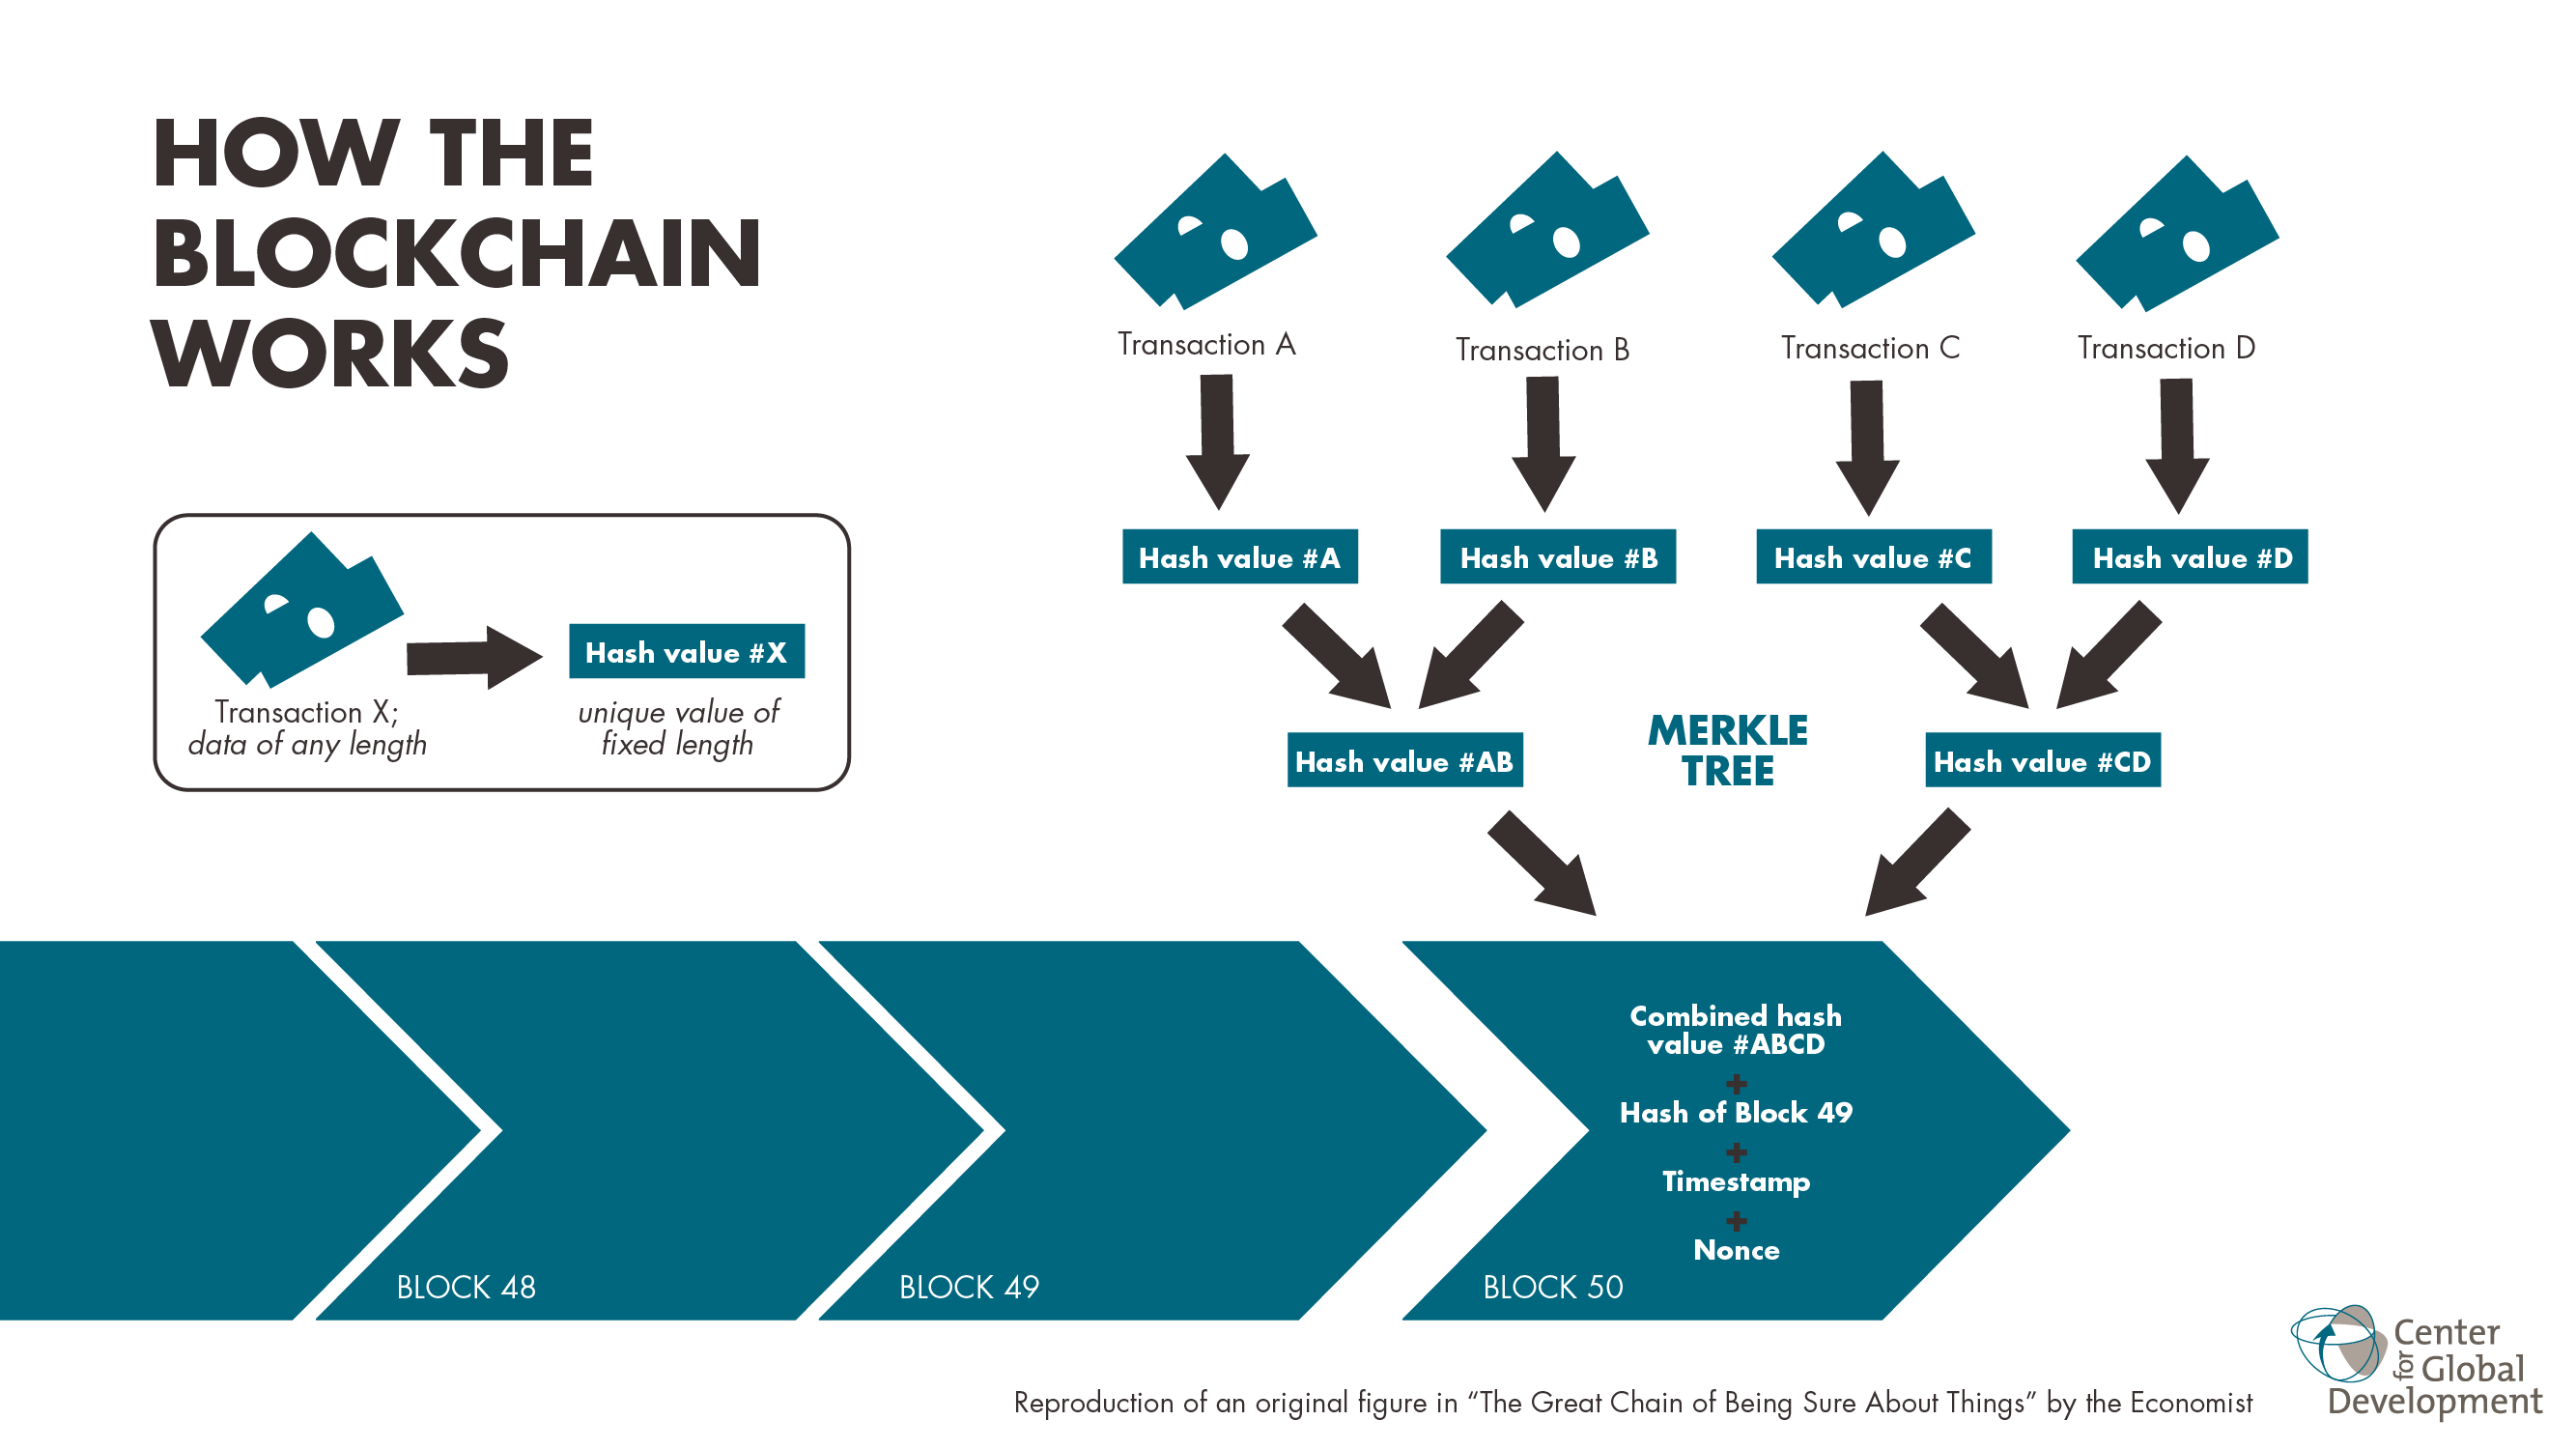
\includegraphics[scale=0.35]{media/Blockchain_workflow.png}
\caption{Representation of a blockchain's structure}
\label{fig:blockchain_workflow}
\end{figure}

\subsection{Immutability}
    This hash thus guarantees that the blocks are linked to each other, but it also guarantees the integrity of the block chain. If one block is altered, the hash on the block that follows it stops matching the block's. If we really wanted to change something on this  first block, we would have to alter the hash on the following block to match. But then, that second block would also have been altered, and we would have to change the hash on the third block to match, and so on. This means that the blockchain is immutable, as it is not possible to alter a single block without manually altering all the others. 
    
\subsection{Consensus}
    The blockchain and its data exists only in a \textbf{peer-to-peer network}, and as such, it is stored and extended by the nodes of the network, which form a topology between them. The nodes are machines that have the core code of the blockchain system and which receive and share among themselves the incoming information, in the form of blocks, validating it according to the established rule set. All the nodes, if they are not malicious and actively attempting to change the contents of the chain, contain the same blockchain structure and information, as they all agree on its contents through a consensus algorithm. 
    
     Some nodes are open to the internet and the world, thus receiving information from outside the peer-to-peer network and disseminating it to the rest of the network's nodes. A subset of the nodes, called miners, will then gather the circulating information from the peer-to-peer network (by receiving transactions from the nodes they are connected to), and form blocks of information, which they try adding to the blockchain. Obviously, it is impossible for all the nodes to add their blocks at the same time, as each of them would then have a different version of the blockchain and they would get desynchronized. And so, the nodes must reach a consensus as to which block gets added next to the blockchain. For this very reason, the code of the blockchain must have both a consensus algorithm and also a block validation algorithm.
     
     In public blockchains, the mining nodes do all the hard work, and they usually need some incentive to do so. Cryptocurrencies are virtual currencies that only exist on the blockchain they belong to, and they allow for a new monetary system to come into life. These currencies play an important role in blockchain, since they allow for miners to be rewarded. Without them, public blockchains would probably not work as well, which is why there are so many alternative currencies popping up, with the advent of this technology. 
     
     Of course, this is just one of many ways to make a blockchain move forward successfully, and other types of consensus algorithms have been idealized, though most of the consensus algorithms in public blockchains will use cryptocurrencies as the prime incentive.
    
    
\subsection{Private, Public and Hybrid Blockchains}

    Blockchain, traditionally, is of public nature. But, as many institutions grew aware of the possible benefits of this technology, they started investing in it, and so appeared the private blockchains and the semi-private or consortium blockchains.
    
    \paragraph{Public Blockchains} When a blockchain is public, it is accessible to any user. Anyone is able to both read and validate information from it, as well as contribute to its extension by participating in the consensus process. They are secured by the economic incentives that are given to the miners, in the form of cryptocurrency tokens. These blockchains can be  considered fully decentralized and have no access control. Every user is at the same level.
    
    \paragraph{Private Blockchains} These are usually owned by some organization and have access control, restricting write access to certain peers inside the organization. Read access might be restricted or not, according to the organization's goals. These blockchains, unlike public ones, might not require cryptocurrency or incentives, as the maintenance of the blockchain is done by the organization who owns it, and so they have all the interest in having nodes that can run the consensus process. In the end, this is a more centralized version of the blockchain, as the nodes are concentrated under the ownership of the organization. This also gives the advantage that alterations to the blockchain are easier to achieve, if so is desired (though it subtracts from the actual meaning and concept of an immutable blockchain). It is usually more efficient than public blockchains, being able of achieving a higher number of transactions processed per second.
    
    \paragraph{Consortium blockchains} They are a kind of hybrid blockchain, though closer to a private blockchain. They are controlled by many different organizations, and the consensus process is handled by pre-selected nodes from the organizations. This consensus might involve, for example, at least a certain percentage of the nodes agreeing on something (e.g.: if there are 15 fixed nodes, require at least 10 to sign the block). The permissions to read might be public or otherwise permissioned, and as such, this can also be considered a partially decentralized blockchain.

    Consortium and private blockchains are not that different. According to Vitalik Buterin,~\cite{Buterin2015}, \textit{"so far there has been little emphasis on the distinction between consortium blockchains and fully private blockchains, although it is important: the former provides a hybrid between the ‘low-trust’ provided by public blockchains and the ‘single highly-trusted entity’ model of private blockchains, whereas the latter can be more accurately described as a traditional centralized system with a degree of cryptographic auditability attached"}.
%--> Hyperledger composer leans more towards the consortium permissioned blockchain type
    \subsection{Types of Consensus Mechanisms and Algorithms}
    
     The most commonly used consensus algorithm is \textbf{Proof of Work (PoW)}, though there are others, like the most used alternatives, \textbf{Proof of Stake (PoS)}, and \textbf{Proof of Activity (PoA)}. We showcase some of the algorithms in Table~\ref{table:consensus_comparison}.
    



%%%%%%%%%%% TABLE

% Please add the following required packages to your document preamble:
% \usepackage[normalem]{ulem}
% \useunder{\uline}{\ul}{}
\begin{table}[]
\centering
\caption{Comparison between different consensus mechanisms.}
\label{table:consensus_comparison}
\begin{tabular}{|l|l|l|}
\hline
Type                                                                       & Overview                                                                                                                                                                                                                                                                                                                                                                                                                                                                                                                                                                                                     & Better Used In                                                                           \\ \hline
Proof of Work (PoW)                                                        & \begin{tabular}[c]{@{}l@{}}In short, PoW works by making the nodes spend \\ computational power until they can find out a hash \\ that satisfies a certain rule, for a certain block. When \\ a node finds this hash, it is allowed to extend the \\ blockchain with that block. The node transmits the \\ new blockchain to all the other nodes. It is assumed \\ that the longed valid chain (where all blocks have \\ valid mininghashes and valid contents) held by any \\ block is the correct one. Additionally, the creator of \\ a block includes a reward for themselves in the block.\end{tabular} & \begin{tabular}[c]{@{}l@{}}Public Blockchains\\ (Bitcoin, alt coins)\end{tabular}        \\ \hline
Proof of Stake (PoS)                                                       & \begin{tabular}[c]{@{}l@{}}In PoS, the "miners" stake their cryptocurrency \\ tokens as a bet, on which block they want to \\ include in the blockchain. By doing so, they \\ actively have a chance to mint that block \\ proportional to the number of tokens they \\ stake. This makes it so that any participant of the \\ network has in its best interest to be honest. The \\ higher their stake, the more invested in the \\ network they are. PoS is less wasteful than PoW, \\ which consumes a lot of energy in computational \\ power.\end{tabular}                                              & \begin{tabular}[c]{@{}l@{}}Public Blockchains,\\ Consortium \\ Blockchains\end{tabular}  \\ \hline
\begin{tabular}[c]{@{}l@{}}Proof of Authority\\ (PoA)\end{tabular}         & \begin{tabular}[c]{@{}l@{}}The transactions are validated, aggregated into blocks \\ and put into the blockchain by approved known nodes,\\  which act like "admins" and are the source of truth \\ for the system. This is a more centralized kind of \\ consensus.\end{tabular}                                                                                                                                                                                                                                                                                                                            & Private Blockchains                                                                      \\ \hline
\begin{tabular}[c]{@{}l@{}}Proof of Elapsed\\ Time (PoET)\end{tabular}     & \begin{tabular}[c]{@{}l@{}}Every participant in the network is assigned a random\\  amount of time to wait, and the first participant to \\ finish waiting gets to commit the next block.\end{tabular}                                                                                                                                                                                                                                                                                                                                                                                                       & \begin{tabular}[c]{@{}l@{}}Private Blockchains,\\ Consortium \\ Blockchains\end{tabular} \\ \hline
\begin{tabular}[c]{@{}l@{}}Byzantine Fault \\ Tolerance (BFT)\end{tabular} & \begin{tabular}[c]{@{}l@{}}There are many algorithms for this kind of consensus.\\ One is Practical BFT (PBFT), with pre-selected nodes \\ selecting and ordering the transactions.\end{tabular}                                                                                                                                                                                                                                                                                                                                                                                                             & \begin{tabular}[c]{@{}l@{}}Private Blockchains,\\ Consortium \\ Blockchains\end{tabular} \\ \hline
\end{tabular}
\end{table}



%%%%%%%%%%% TABLE END

\subsection{Transparency}
   The blockchain is not only available to the mining nodes in the network. Though they are the ones who actively interact with the chain in order to make it grow, if the chain is public, anyone can view the records and verify the authenticity of the data. This is the property of transparency. In private or permissioned blockchains, it might happen that only certain actors have access to certain records, according to the access control rules set by the organization or set of organizations that manage it. This is done with the help of sets of asymmetric key pairs and a public key infrastructure.
    
% Talk about merkle tree - is it necessary?


%\section{Security Features}
%In a blockchain, security is a multi-faceted aspect. It depends heavily on cryptography, especially hashing and public key cryptography. But it also depends on a blockchain's characteristics and set values, such as the average block time.
%\paragraph{Hashing}
%\paragraph{Public Key Cryptography}
%\paragraph{Other aspects and concerns}

\section{Applications}

    In general, blockchains are applied in different ways, from public ledgers to private, in a continuum, according to the specific needs. Many of them even apply the concept of smart contracts. Vitalik himself suggested some possible applications of Ethereum, and many more have been idealized, with some even being successfully applied. Here are some examples of areas where the benefits of introducing blockchain have been studied.
    

%{It could make sense to mention, for each of the aread below, the key properties of a blockchain that it expectedly benefits from.} -> In the frameworks chapter, it is mentioned a bit better than here, but it is probably not essential for what we want here. We already decided that SCM is our focus

    \begin{itemize}
     \item Identity/Record Management - like in a notary, documents are validated and recorded.
     
     \item Insurance - Smart contracts, having to abide to certain rule with certainty, make for a perfect system for risk-management. Given that certain conditions are met, the insurance could be claimed, giving way to faster and less error-prone insurance processing.
     
     \item Health care - Health records easily accessible anywhere. This could be coupled with other applications, like using sensors and smart contracts to automatically monitor patient status.
     
     \item Distributed Cloud Storage - Instead of the traditional centralized cloud, distributed clouds could become a reality.
     
     \item Voting - Using blockchain, digital voting could become feasible. The greatest barrier to e-voting have been the concerns with security, and blockchain provides an anonymous and secure way to do it.
     
     \item Internet-of-Things (IoT) - Any object connected to the Internet can upload information, which can either be stored or processed on the blockchain. Devices with sensors, for instance, can be programmed to send their values to the blockchain, which can then be queried by others to check these values. There can even be pre-programmed smart contracts that have events based on what is happening and the information that is being sent by the devices.
	\end{itemize}
